% Following the previous findings, this chapter will research and implement a Recurrent Neural Network using voltage, current, temperature and the known state of a battery charge to predict and feed forward the outputted result.
% It meant to use methodology constructed from the previous chapter:
% \begin{itemize}
%     \item Use single-cell data over the entire temperature range for a single profile, use FUDS for better performance capture.
%     \item Train a model with recommended modifications.
%     \item Verify the model against another cell with the same profile.
%     \item Validate the performance against the other two profiles, DST and US06.
% \end{itemize}

%
%
%There have been several attempts to determine the most effective strategy for model training.
%Both LSTM and Gradient Recurrent Unit are effective, and there is no noticeable difference in the impact between speed and outputted accuracy.


%
%

%
%
% The rest of this paper is organised as follows: a methodology for an RNN model discussed in Section 2.
% The details of how auto-regression has been utilised are in Section 3.
% Subsections 4.1 and 4.2 separate points of model validation and process of parameter estimation.
% Finally, section 5 concludes the research by outlining several observations, which may require separate consideration.
% Most were isolated to closed scenarios with provided data or from battery cycling machines.
% The most promising approach to improve a model and make it more universal is to increase complexity. While some introduced deeper layer networks, others added additional mechanisms to those already used.
% \begin{landscape}
%     \begin{figure}[ht]
%         \centering
%         % 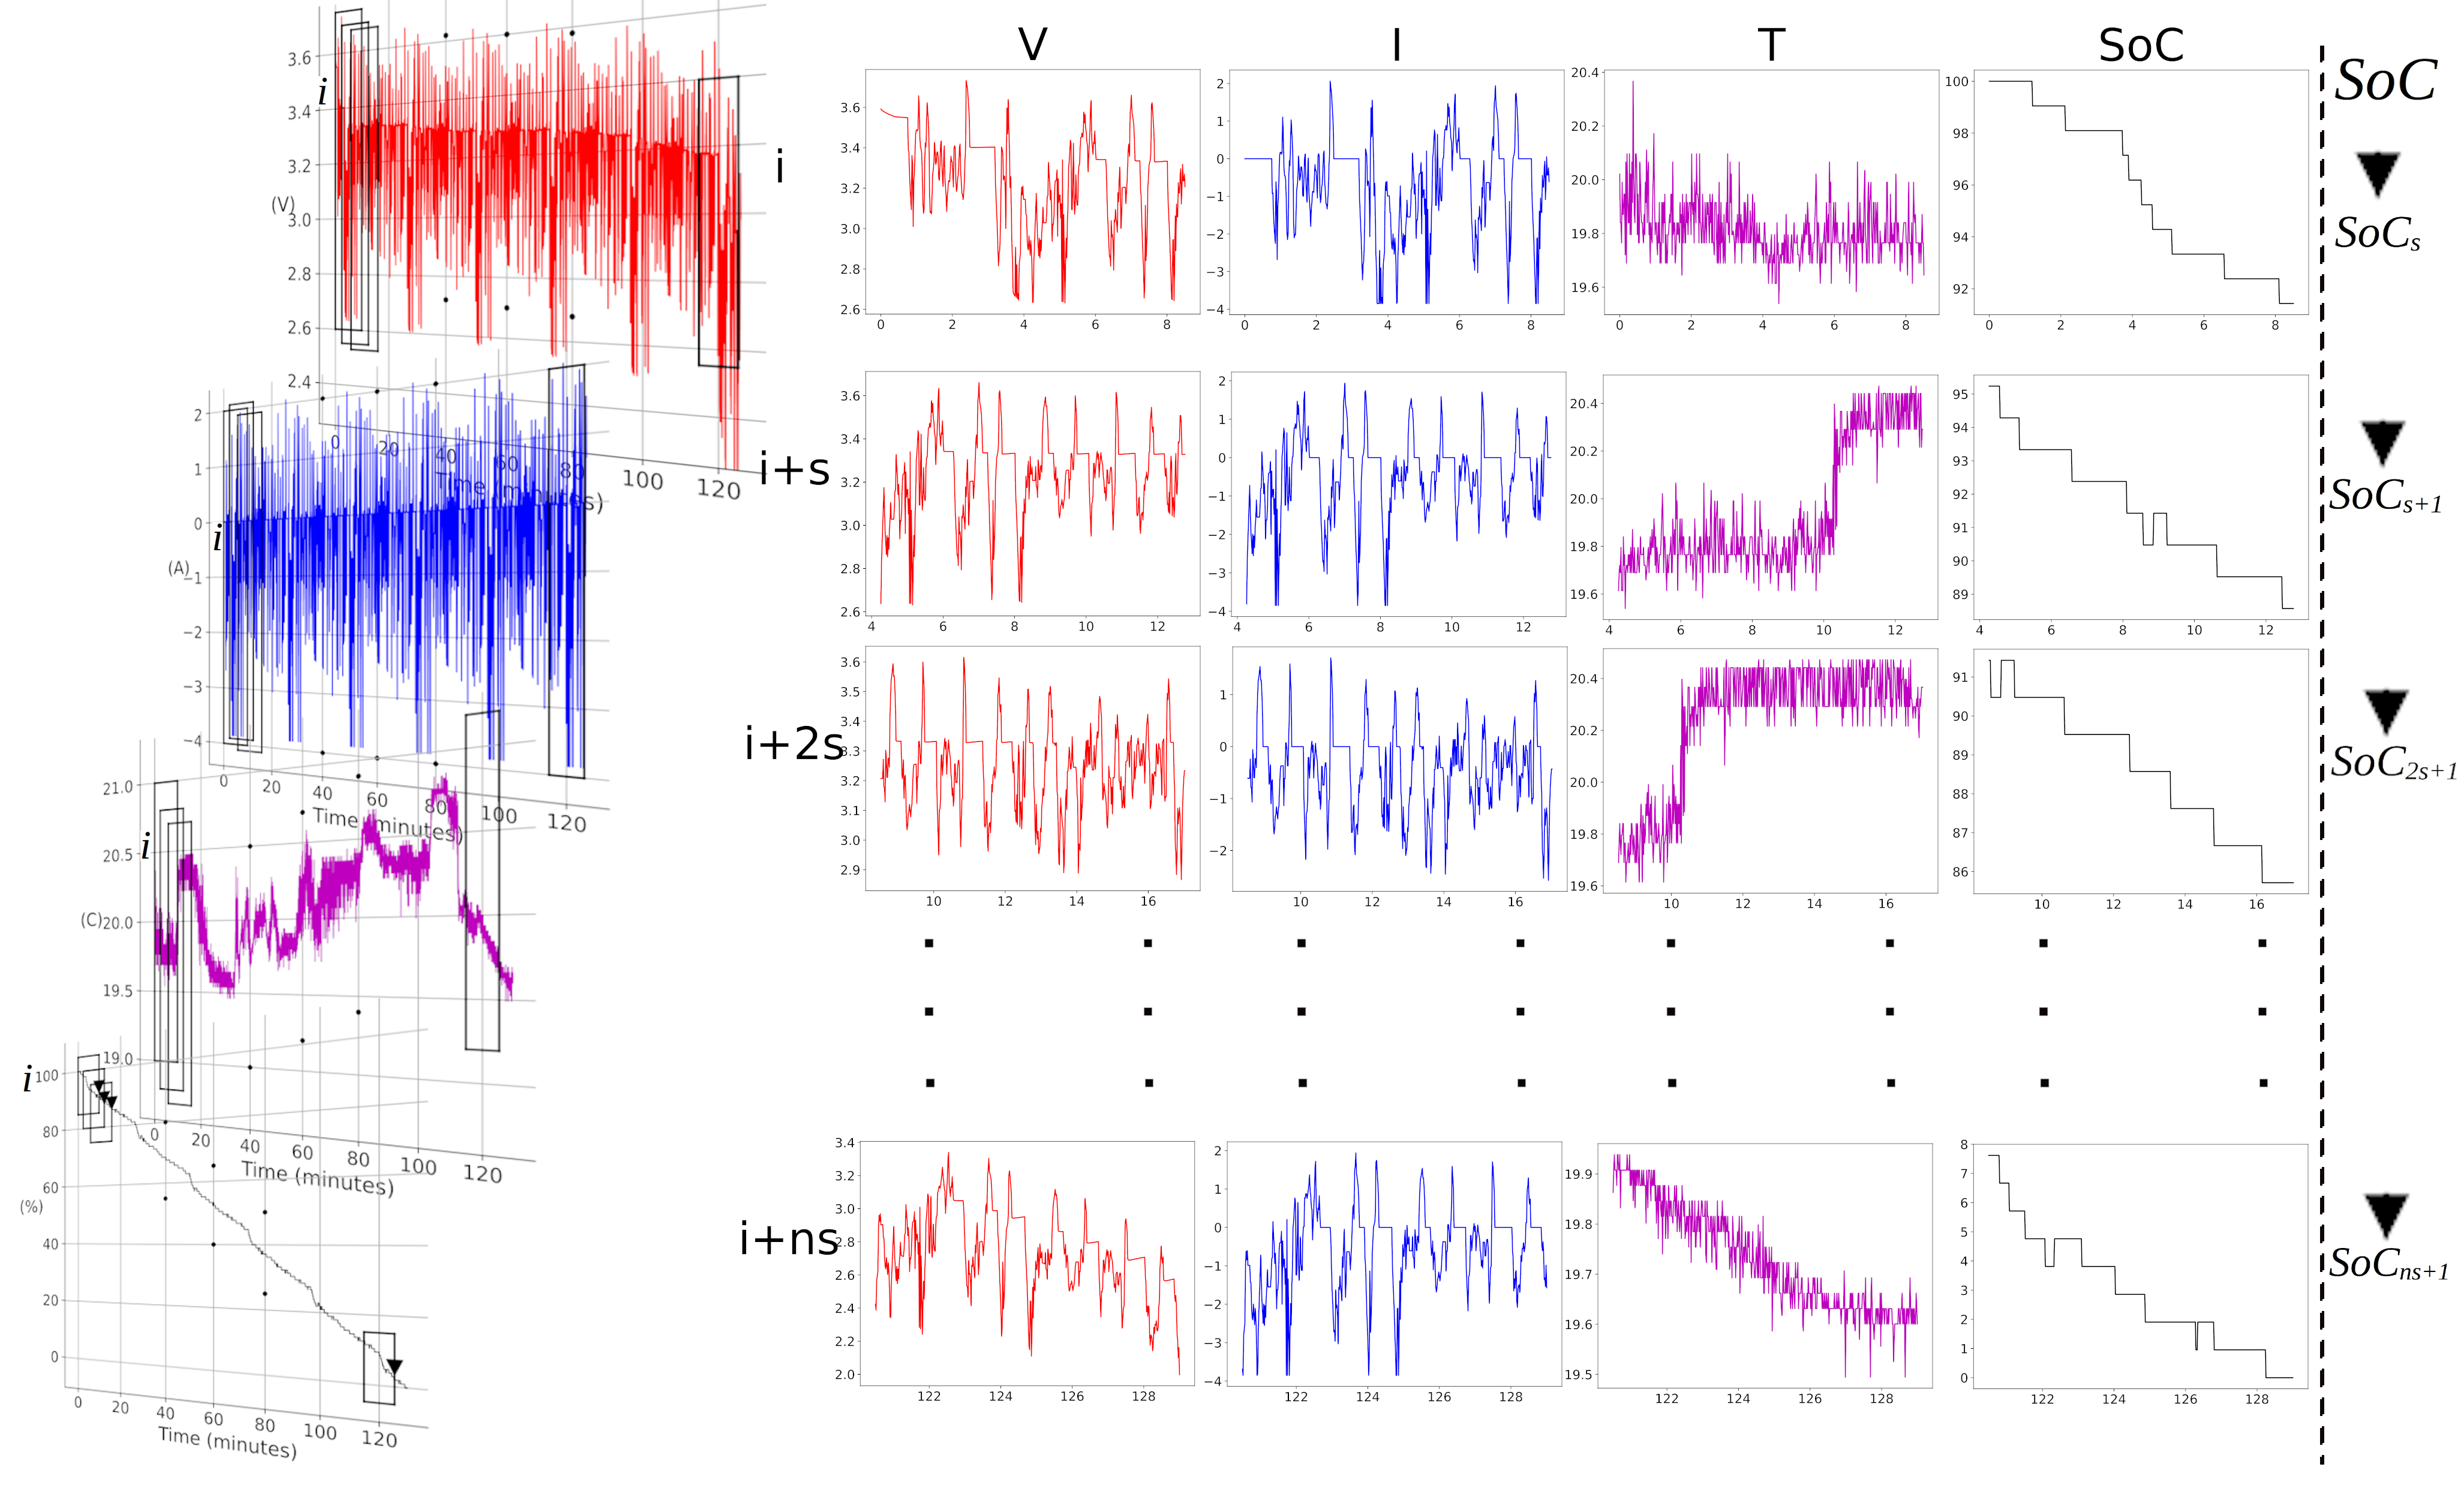
\includegraphics[width=0.9\linewidth]{II_Body/images/Windowing3D-1.jpg}
%         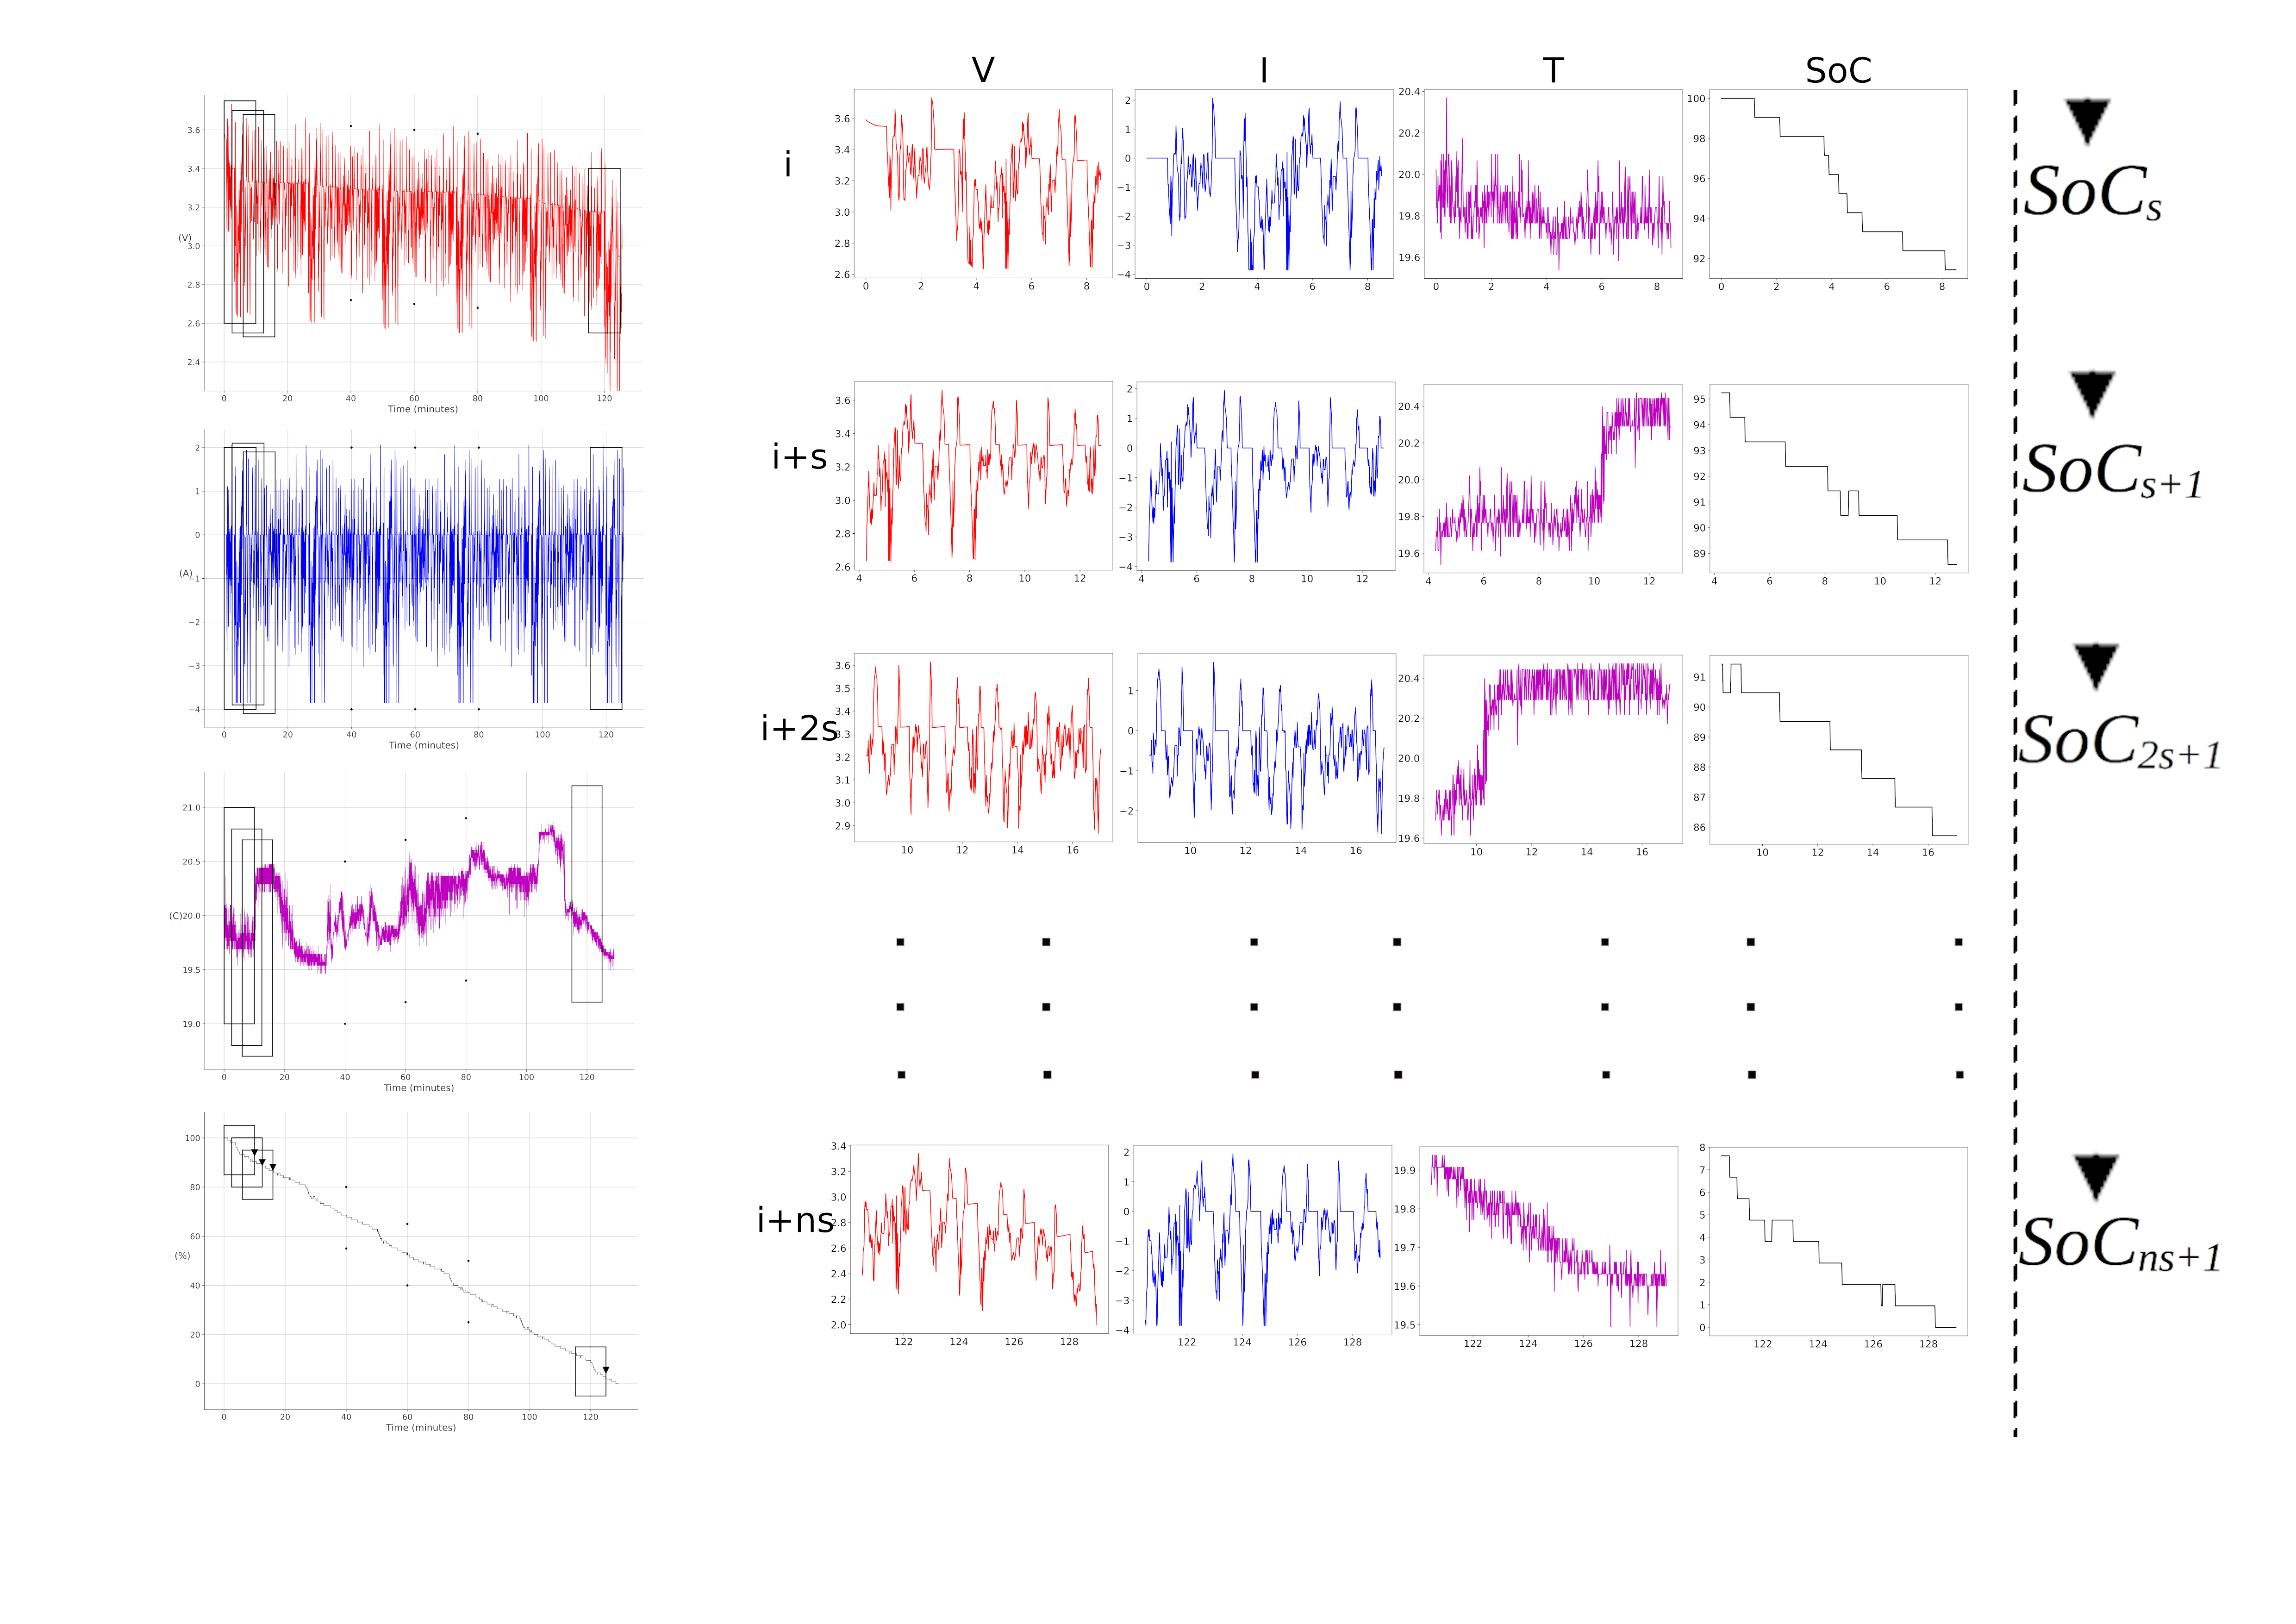
\includegraphics[width=0.9\linewidth]{II_Body/images/Windowing4f-A3.jpg}
%         \caption{Data Windowing scheme at 1Hz sampling rate with four features and one output. For visualisation purposes, the $s$-step has been used as 250 seconds, which is different from the actual implementation. The initial index $i$ was kept as a value close to the beginning of the data, around zero.}
%         \label{fig:Windowing}
%     \end{figure}
% \end{landscape}